\documentclass[10 pt]{article}

\usepackage[OT2]{fontenc}
\usepackage[serbian]{babel}
\usepackage[top= 27mm, bottom=27mm, left=25mm, right=25mm]{geometry}
\usepackage{amsmath}
\usepackage{amssymb}
\usepackage{amsthm}
\usepackage{graphicx}
\usepackage{float}
\usepackage{caption}
\usepackage{subfig}
\usepackage{hyperref}
\usepackage{indentfirst}
%\usepackage{enumitem}
%\setlist[enumerate]{label*=\arabic*.}

\renewcommand*\contentsname{Sadrzhaj:}
\renewcommand{\figurename}{Slika}
\renewcommand{\refname}{Literatura}

\hypersetup{
    colorlinks=true,
    linktoc=all,
    linkcolor=blue,
}


\title{\vspace*{\fill}\huge{\textbf{Grupni projektni rad\\ 
		\vspace{10 pt} Informacioni sistem za iznoshenje smec1a}}}
\date{}
\author{}

\begin{document}

\maketitle	

\
\\[270 pt]
\
\begin{flushleft}
	Studenti:\hspace{260 pt} Predmet: Informacioni sistemi\\ 
	Miroslav Mishljenovic1\hspace{197 pt} Profesor: Sasha Malkov\\
	Filip Lazic1\hspace{244 pt} Asistent: Aleksandra Kocic1\\
	Nemanja Antic1\\
	Marija Mijailoic1 
 \end{flushleft}

 \
 \\[50 pt]
 \
\begin{center}
  Univerzitet u Beogradu, Matematichki fakultet
  \\ novembar 2017. godine
\end{center}

\thispagestyle{empty}

\newpage
\tableofcontents

\newpage
\section{Uvod}

\subsection{Kratak opis sistema}
\setlength{\parindent}{30pt} Sistem za iznoshenje otpada funkcionishe tako shto se razne vrste otpada odlazhu na za tu vrstu predvidjen nachin. Sistem omoguc1ava iznoshenje razlichitih vrsta otpada kao shto su gradjevinski, reciklazhni, elektrichni, itd … Takodje sistem omoguc1ava prac1enje radnika na terenu koji rade na procesu iznoshenja i odlaganja otpada(radnici, vozachi…). Deo sistema c1e se baviti naplac1ivanjem usluga. U okviru sistem podrazumeva da postoji sistem za reciklazhu, i magacin za skladishtenje otpada.  

\subsection{Akteri}
	\begin{enumerate}
		\item
			\textit{\textbf{Klijent}} je subjekat chiji se otpad odlazhe. Mozhe biti redovan pretplatnik usluga iznoshenja smec1a ili firma koja trazhi ekspilicitno iznochenje otpada(naplac1uje se po posebnom sistemu naplate).
		\item 
			\textit{\textbf{Dispecher}} prikuplja zahteve klijenata.
		\item 
			\textit{\textbf{Koordinator}} u skladu sa resursima kojima sluzhba raspolazhe pravi radne naloge.
		\item 
			\textit{\textbf{Radnici}} sprovode zadatke koje postavlja koordinator. Mozhe biti vozach, radnik na rukovanju kontejnerima, itd …
		\item 
			\textit{\textbf{Magacioner}} skladishti otpad u magacin. 
		\item
			\textit{\textbf{Upravnik}} je zaduzhen da vodi evidenciju o statusu radnika, i upravlja prodajom otpada iz magacina.
	\end{enumerate}


\section{Analiza sistema}
\setlength{\parindent}{30pt} Postojec1i sistem sadrzhi prevelik broj zaposlenih u administraciji. Ovaj sistem je napravljen sa pokushajem da smanji broj ljudi u administraciji i sistem uchini jednako efikasnim. Takodje, u odnosu na prethodni sistem nash podrazumeva i savremeniju opremu za rad. Prikaz informaciong sistema dat je na slici \ref{fig:dijagramKonteksta} i \ref{fig:dijagramTokaPodataka}. 

\subsection{Dijagram celog sistema}
	\begin{figure}[H]
		\centering
		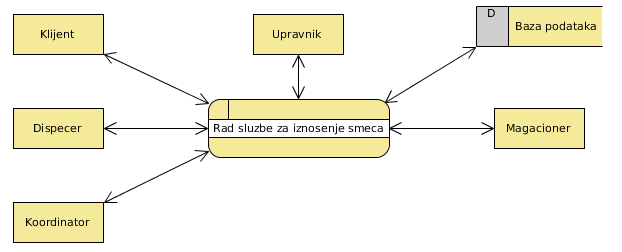
\includegraphics[width=15cm,height=15cm,keepaspectratio]{slike/DijagramKonteksta}\\
		\caption{Dijagram konteksta	\label{fig:dijagramKonteksta}}
	\end{figure}
	
	\begin{figure}[H]
		\centering
		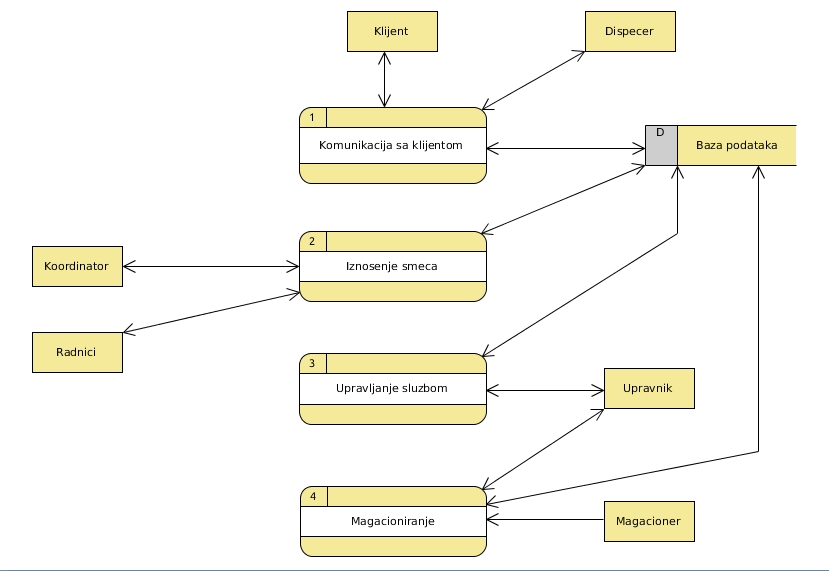
\includegraphics[width=15cm,height=15cm,keepaspectratio]{slike/DTP.png}\\
		\caption{Dijagram toka podataka	\label{fig:dijagramTokaPodataka}}
	\end{figure}
	
\section{Sluchajevi upotrebe}


	\subsection{Komunikacija sa klijentom}
	
	\begin{figure}[H]
		\centering
		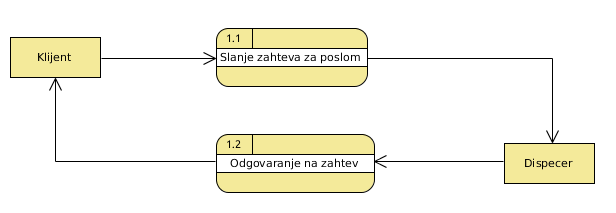
\includegraphics[width=15cm,height=15cm,keepaspectratio]{slike/KomunikacijaSaKlijentom.png}\\
		\caption{Dijagram Komunikacije sa klijentom}
	\end{figure}
	
	\subsubsection{Sluchaj uptrebe - Slanje zahteva za poslom}
		\begin{itemize}
			
			\item \textit{Kratak opis} - Klijent mozhe da kontaktira sluzhbu preko online formulara ili telefonom.
			
			\item \textit{Uchesnici}
				\begin{enumerate}
					\item Klijent
					\item Dispecher
				\end{enumerate}
			
			\item \textit{Preduslovi} - Nema
			
			\item \textit{Postuslovi} - Dispecher je uspeshno evidentirao zahtev klijenta.
			
			\item \textit{Osnovni tok}
				\begin{enumerate}
					\item Klijent kontaktira sluzhbu
					\item Dispecher evidentira zahtev
				\end{enumerate}
			
			\item \textit{Alternativni tokovi} - U sluchaju nepravilnosti u formularu, dispecher kontaktira klijenta da koriguje zahtev.
			
			\item \textit{Podtokovi} 
				\begin{enumerate}
					\item Klijent kontaktira sluzhbu: 
					\begin{enumerate}
						%\setcounter{enumi}{1}
						\item Klijent popunjava online formular
						\item Klijent poziva dispechera
					\end{enumerate}
				\end{enumerate}
			
			\item \textit{Specijalni zahtevi} - Nema
			
			\item \textit{Dodatne informacije} - Nema
			
		\end{itemize}
		
	\subsubsection{Sluchaj uptrebe - Odgovaranje na zahtev}
	\begin{itemize}
		
		\item \textit{Kratak opis} -  Dispecher proverava da li posao mozhe da se obavi ove nedelje. Ako mozhe obaveshtava klijenta o vremenu izvrshavanja, u suprotnom ga obaveshtava da se posao odlazhe do daljnjeg.
		
		\item \textit{Uchesnici}
		\begin{enumerate}
			\item Klijent
			\item Dispecher
		\end{enumerate}
		
		\item \textit{Preduslovi} - Zahtev je pravilno podnet i koordinator je obradio zahtev.
		
		\item \textit{Postuslovi} - Klijent je obaveshten o stanju njegovog zahteva.
		
		\item \textit{Osnovni tok}
		\begin{enumerate}
			\item Dispecher proverava stanje baze
			\item Dispecher kontaktira klijenta
		\end{enumerate}
		
		\item \textit{Alternativni tokovi} - Nema
		
		\item \textit{Podtokovi} 
		\begin{enumerate}
				\item Dispecher kontaktira klijenta
				\begin{enumerate}
				%	\setcounter{enumi}{2}
					\item Dispecher obaveshtava klijenta o vremenu izvrshavanja posla
					\item Dispecher obaveshtava klijenta o odlaganju posla
				\end{enumerate}
		\end{enumerate}
		
		\item \textit{Specijalni zahtevi} - Nema
		
		\item \textit{Dodatne informacije} - Nema
		
	\end{itemize}
	
	%----------------------------------------------------------------

	\subsection{Iznoshenje smec1a}
	
	\begin{figure}[H]
		\centering
		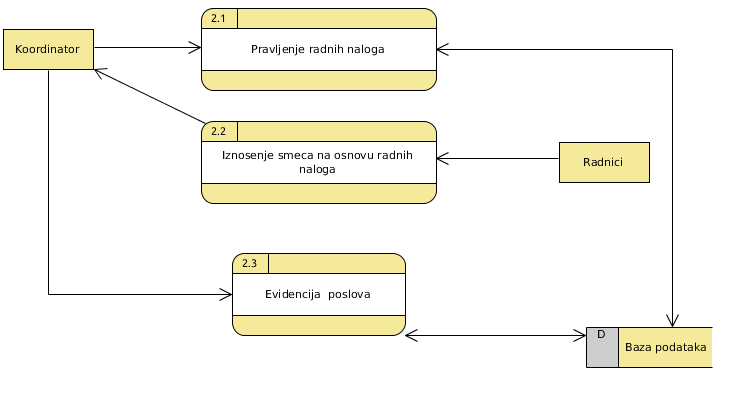
\includegraphics[width=15cm,height=15cm,keepaspectratio]{slike/IznosenjeSmeca.png}\\
		\caption{Dijagram iznoshenja smec1a}
	\end{figure}
	
	\subsubsection{Sluchaj uptrebe - Pravljenje radnih naloga}
	\begin{itemize}
		
		\item \textit{Kratak opis} - Koordinator na osnovu podataka iz baze kreira radne naloge.
		
		\item \textit{Uchesnici}
		\begin{enumerate}
			\item Koordinator
		\end{enumerate}
		
		\item \textit{Preduslovi} - U bazi su azhurirane informacije o poslovima i radnicima.
		
		\item \textit{Postuslovi} - Kreirani su radni nalozi.
		
		\item \textit{Osnovni tok}
		\begin{enumerate}
			\item U bazi provera spisak poslova i raspolozhivost radne snage
			\item Kreira radne naloge
			\item Azhurira bazu
		\end{enumerate}
		
		\item \textit{Alternativni tokovi} - Nema
		
		\item \textit{Podtokovi} - Nema
		
		\item \textit{Specijalni zahtevi} - Nema
		
		\item \textit{Dodatne informacije} - Nema
		
	\end{itemize}
	
	\subsubsection{Sluchaj uptrebe - Iznoshenje smec1a na osnovu radnih naloga}
	\begin{itemize}
		
		\item \textit{Kratak opis} - Radnici preuzimaju radne naloge i izlaze na teren, Obaveshtavaju koordinatora o stanju na terenu.
		
		\item \textit{Uchesnici}
		\begin{enumerate}
			\item Koordinator
			\item Radnici
		\end{enumerate}
		
		\item \textit{Preduslovi} - Izdati su radni nalozi.
		
		\item \textit{Postuslovi} - Koordinator je obaveshten o ishodu posla.
		
		\item \textit{Osnovni tok}
		\begin{enumerate}
			\item Radnici preuzimaju radne naloge.
			\item Radnici izlaze na teren.
			\item Radnici obaveshtavaju koordinatora o ishodu posla.
		\end{enumerate}
		
		\item \textit{Alternativni tokovi} - Nema
		
		\item \textit{Podtokovi} - Nema
		
		\item \textit{Specijalni zahtevi} - Nema
		
		\item \textit{Dodatne informacije} - Nema
		
	\end{itemize}
	
	\subsubsection{Sluchaj uptrebe - Evidentiranje poslova}
	\begin{itemize}
		
		\item \textit{Kratak opis} - Koordinator evidentira u bazi koji su radnici trenutno zauzeti poslom i po avrshetku posla ih oslobadja. Takodje evidentira iu bazi uspeshnost poslova.
		\item \textit{Uchesnici}
		\begin{enumerate}
			\item Koordinator
		\end{enumerate}
		
		\item \textit{Preduslovi} - Nema
		
		\item \textit{Postuslovi} - Azhurirana je baza.
		
		\item \textit{Osnovni tok}
		\begin{enumerate}
			\item Koordinator evidentira u bazi zauzetost radnika
			\item Koordinator evidentira u bazi uspeshnost poslova
		\end{enumerate}
		
		\item \textit{Alternativni tokovi} - Nema
		
		\item \textit{Podtokovi} - Nema
		
		\item \textit{Specijalni zahtevi} - Nema
		
		\item \textit{Dodatne informacije} - Nema
		
	\end{itemize}
	
	%-------------------------------------------------------------

	\subsection{Upravljanje sluzhbom}
	
	\begin{figure}[H]
		\centering
		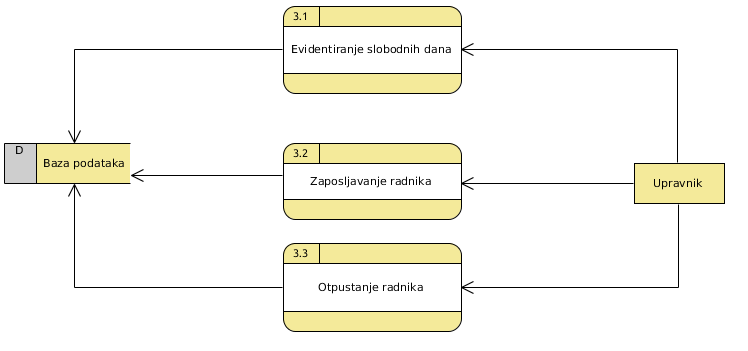
\includegraphics[width=15cm,height=15cm,keepaspectratio]{slike/UpravljanjeSluzbom.png}\\
		\caption{Dijagram upravljanja sluzhbom}
	\end{figure}
	
	\subsubsection{Sluchaj uptrebe - Evidentiranje slobodnih dana}
	\begin{itemize}
		
		\item \textit{Kratak opis} - Upravnik evidentira u bazi da je radnik na odmoru ili se vrac1a na posao.
		
		\item \textit{Uchesnici}
		\begin{enumerate}
			\item Upravnik
		\end{enumerate}
		
		\item \textit{Preduslovi} - Radnik ima jos slobodnih dana ili mu je isteklo vreme odmora.
		
		\item \textit{Postuslovi} -Radnik je na odmoru ili se vrac1a na posao.
		
		\item \textit{Osnovni tok}
		\begin{enumerate}
			\item Upravnik shalje radnika na odmor
		\end{enumerate}
		
		\item \textit{Alternativni tokovi} - Nema
		
		\item \textit{Podtokovi} - Nema
		
		\item \textit{Specijalni zahtevi} - Nema
		
		\item \textit{Dodatne informacije} - Nema
		
	\end{itemize}
		
	%--------------------------------------------------------------

	\subsection{Magacioniranje}

	\begin{itemize}
		
		\item \textit{Kratak opis} - Magacioner se bavi skladishtenjem robe u magacinu. Upravnik upravlja prodajom artikala iz magacina.
		
		\item \textit{Uchesnici}
		\begin{enumerate}
			\item Upravnik
			\item Magacioner
		\end{enumerate}
		
		\item \textit{Preduslovi} - Radinici su doneli robu na skladishtenje.
		
		\item \textit{Postuslovi} - Roba je upisana u bazu.
		
		\item \textit{Osnovni tok}
		\begin{enumerate}
			\item Magacioner skladishti robu
		\end{enumerate}
		
		\item \textit{Alternativni tokovi} - Nema
		
		\item \textit{Podtokovi} - Nema
		
		\item \textit{Specijalni zahtevi} - Nema
		
		\item \textit{Dodatne informacije} - Nema
		
	\end{itemize}
	
	%------------------------------------------------------
	
\section{Administracija sistema}

\section{Klase podataka}

\section{Prototipovi}
\section{Zakljuchak}
\section{Reference}

\end{document} 